\documentclass[12pt,a4paper]{article}

\input{/home/tabaka/Documents/GitHub/Defs/defs.tex}

\setcounter{zadaniaRozdzial}{1}
\pagestyle{empty}

\begin{document}
	
	\ZbiorZadanie{Poniżej przedstawiono tabele wartości odżywczych (od lewej) kawy, chleba żytniego oraz miodu.
		
		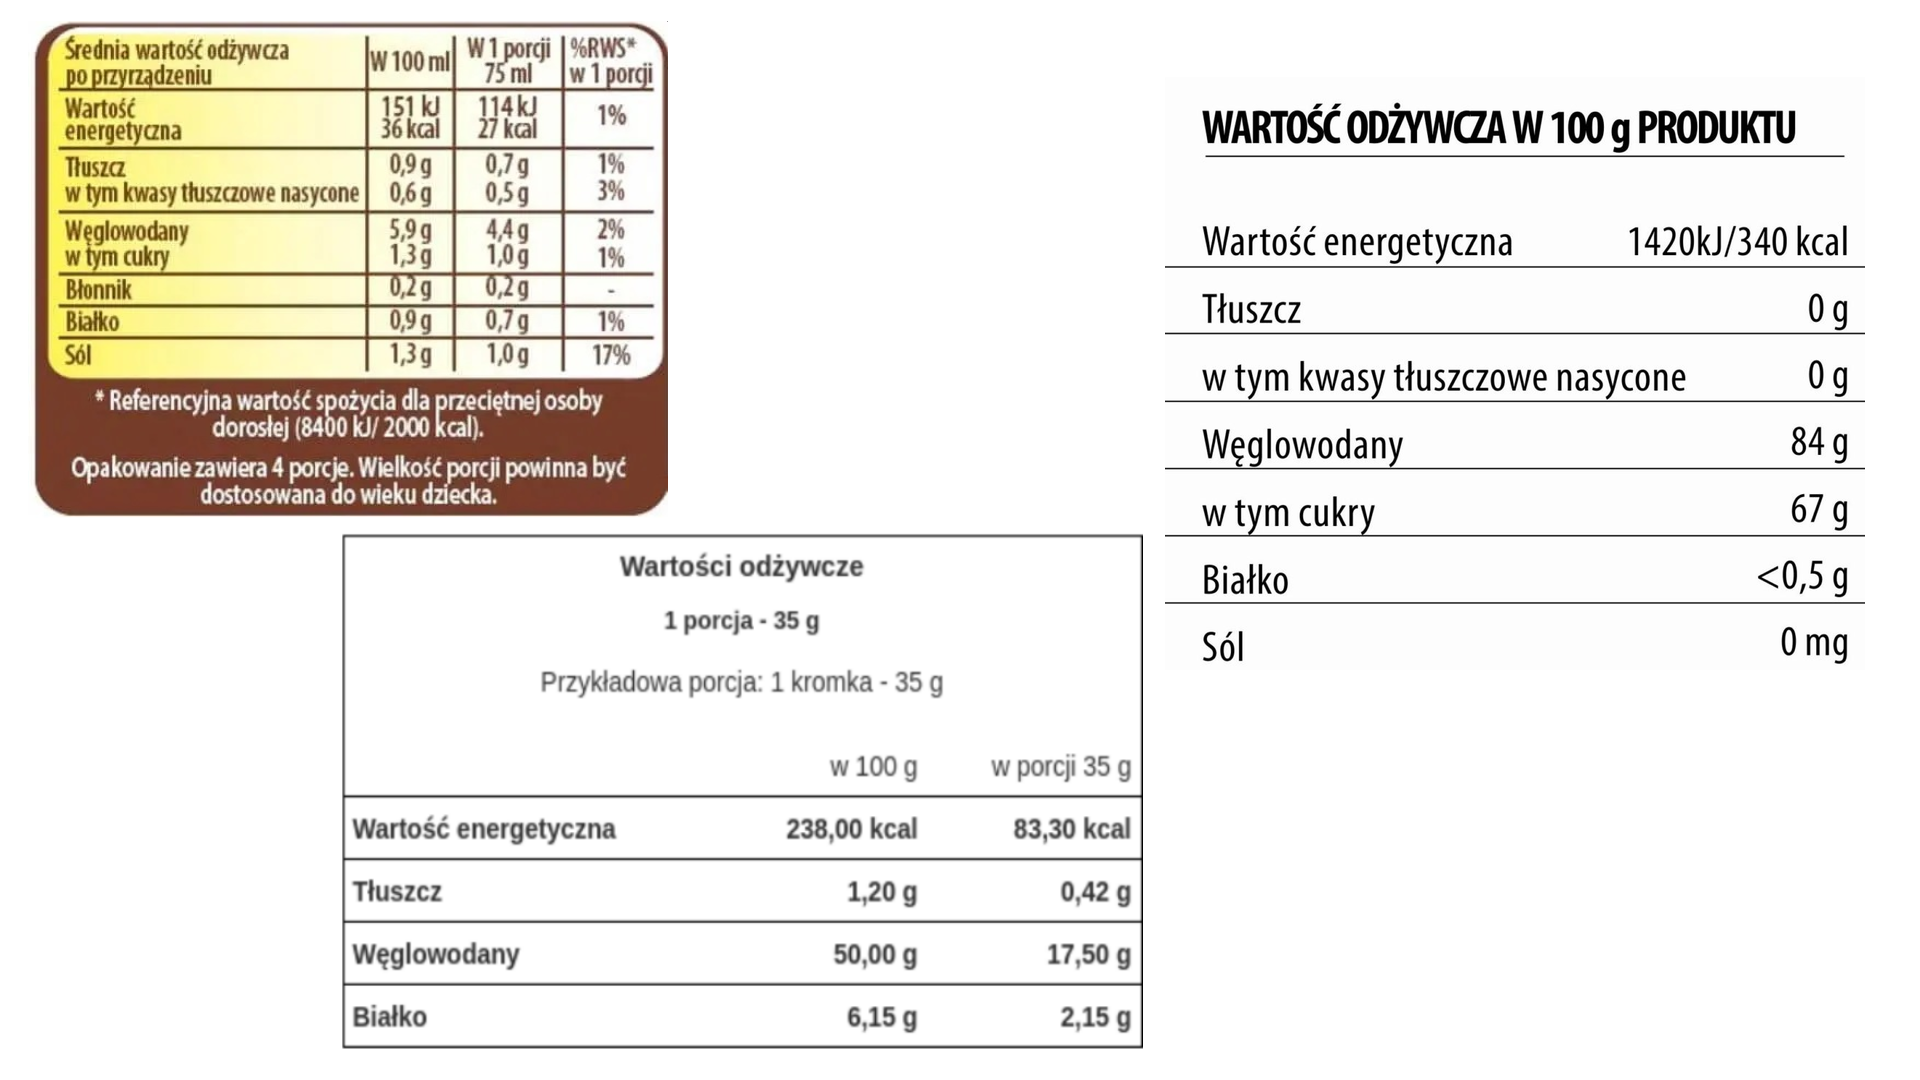
\includegraphics{Kalorie}
		
		\begin{enumerate}[a)]
			\item Ile kalorii ma śniadanie składające się z 300 ml kawy, 2 kromek chleba z 30 g miodu?
			\item Gdzie jest więcej węglowodanów: w kromce chleba czy w 20 g miodu?
			\item Ile gramów miodu należy zjeść, aby dostarczyć organizmowi tyle samo węglowodanów, ile zawierają dwie kromki chleba?
			\item Ile mililitrów kawy należy wypić, aby dostarczyć organizmowi tyle samo kalorii, ile dostarczają dwie kromki chleba?
			\item O ile więcej kalorii dostarcza 100 g chleba niż 100 g miodu?
	\end{enumerate}}

	\ZbiorZadanieTwoXTwo{Zaokrąglij do jedności:}{$17{,}432$}{$12{,}8$}{$0{,}6$}{$35{,}5$}
	
	\ZbiorZadanieTwoXTwo{Zaokrąglij do części dziesiątych:}{$3{,}4701$}{$8{,}9222$}{$12{,}058$}{$0{,}84$}
	
	\ZbiorZadanieTwoXTwo{Zaokrąglij do części setnych:}{$4{,}376$}{$15{,}824$}{$0{,}995$}{$23{,}(73)$}
	
	\ZbiorZadanieTwoXTwo{Zaokrąglij do części tysięcznych:}{$2{,}4738$}{$6{,}1254$}{$0{,}9996$}{$14{,}(37)$}
	
\end{document}